\documentclass{standalone}
\usepackage{tikz}
\begin{document}

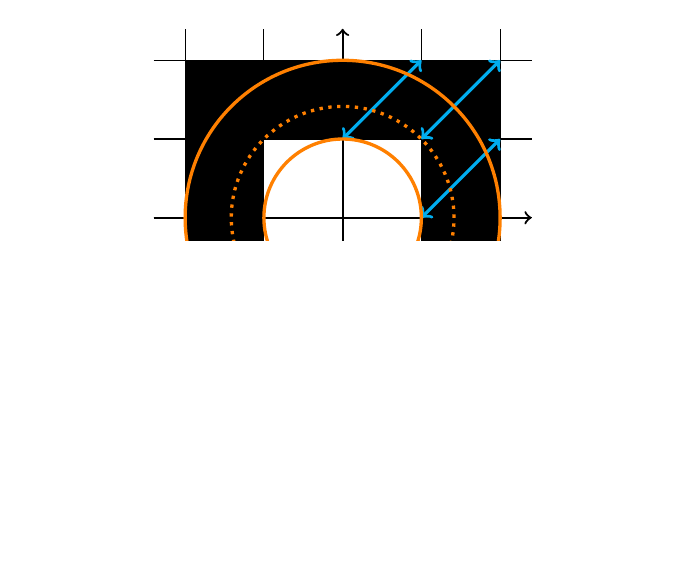
\begin{tikzpicture}
	\newcommand\overhang{0.4};
	\newcommand\xmin{-2};
	\newcommand\xmax{2};
	\newcommand\ymin{-3};
	\newcommand\ymax{2};

	\fill (-2,-2) rectangle (2,2);
	\fill[white] (-1,-1) rectangle (1,1);

	\foreach \i in {\xmin,...,\xmax} {
		\draw (\i, \ymin-\overhang) -- (\i, \ymax+\overhang);
	}
	\foreach \i in {\ymin,...,\ymax} {
		\draw (\xmin-\overhang, \i) -- (\xmax+\overhang, \i);
	}
	\draw[thick,->] (0,\ymin-\overhang) -- (0,\ymax+\overhang);
	\draw[thick,->] (\xmin-\overhang,0) -- (\xmax+\overhang,0);

	\draw[cyan,very thick,<->] (1,0) -- (2,1);
	\draw[cyan,very thick,<->] (0,1) -- (1,2);
	\draw[cyan,very thick,<->] (1,1) -- (2,2);
	
	\draw[orange,very thick] (0,0) circle (1);
	\draw[orange,very thick] (0,0) circle (2);

	\draw[orange,dotted,very thick] (0,0) circle ({sqrt(2)});

	\fill[white] (-4,-.3) -- (4,-.3) -- (4,-4) -- (-4,-4) -- cycle;
\end{tikzpicture}

\end{document}
